%%%%%%%%%%%%%%%%%%%%%%%%%% lecture-1
\begin{frame}
  \frametitle{lecture-1 主要内容}
  \tableofcontents[hideallsubsections]
\end{frame}

\section{课程介绍}

\begin{frame}{课程内容}
\begin{itemize}
	\item 计算机导论:了解计算机的基本知识;掌握计算机操作基本技能。
	\item 程序设计:掌握结构化程序设计方法。会读、会编、会调试C语言程序。
	\item 教材
	\begin{itemize}
		\item 大学计算机,龚尚福, 贾澎涛,西安电子科技大学出版社
		\item C程序设计第五版, 谭浩强,清华大学出版社
	\end{itemize}
\end{itemize}
\end{frame}

\begin{frame}{考核}
\begin{enumerate}
	\item 导论部分计算机应用成绩(C1): 10\%。计算机基本操作技能。
	\item 导论部分课程报告成绩(C2): 10\%。撰写课程学习小论文。
	\item 单元测验成绩(C3、C4): 40\%。根据机试系统给出的练习题目编写程序,通过调试得到正确结果并通过机试系统提交。
	\item 平时作业成绩(C5): 10\%。主要考核对每堂课知识点的复习、理解和掌握程度。
	\item 期末考试成绩(C6): 30\%。主要考程序设计思想、逻辑思维、程序设计方法、程序调试能力。\textbf{考试形式为机试}。
\end{enumerate}
\end{frame}

\section{导论简介}

\begin{frame}{计算机导论主要内容}
总体要求: 了解计算机的基本知识;掌握计算机操作基本技能。\\
\begin{itemize}
	\item 计算机系统组成
	\item 计算机工作原理
	\item 操作系统
	\item 字处理: Microsoft Word
	\item 电子表格: Microsoft Excel
	\item 演示文稿: Microsoft PowerPoint
\end{itemize}
\end{frame}

\begin{frame}{计算机工作原理}
工作原理: ``存储程序''+``程序控制''
\begin{enumerate}
	\item 以二进制方式表示数据和指令
	\item 将程序存入存储器中,由控制器自动读取并执行
	\item 外部存储器$\implies$程序和所需数据$\implies$计算机内存$\implies$在程序控制下由CPU周而复始地取出指令、分析指令、执行指令$\implies$操作完成。	
\end{enumerate}
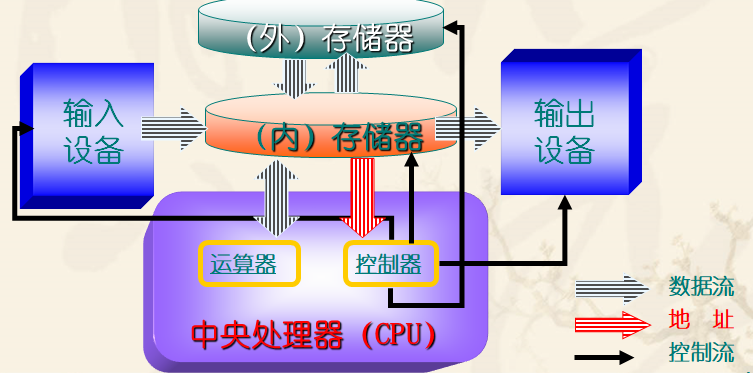
\includegraphics[scale=0.25]{hframe}
\end{frame}

\begin{frame}[shrink]
\frametitle{10,2,16进制的幂展开式}
\begin{align*}
(D)_{10}&=D_{n-1}\times 10^{n-1}+D_{n-2}\times 10^{n-2}+\cdots+D_{1}\times 10^{1}+D_{0}\times 10^{0}\\
&+D_{-1}\times 10^{-1}+D_{-2}\times 10^{-2}+\cdots+D_{-m+1}\times 10^{-m+1}+D_{-m}\times 10^{-m}\\
(B)_{2}&=B_{n-1}\times 2^{n-1}+B_{n-2}\times 2^{n-2}+\cdots+B_{1}\times 2^{1}+B_{0}\times 2^{0}\\
&+B_{-1}\times 2^{-1}+B_{-2}\times 2^{-2}+\cdots+B_{-m+1}\times 2^{-m+1}+B_{-m}\times 2^{-m}\\
(H)_{2}&=H_{n-1}\times 16^{n-1}+H_{n-2}\times 16^{n-2}+\cdots+H_{1}\times 16^{1}+H_{0}\times 16^{0}\\
&+H_{-1}\times 16^{-1}+H_{-2}\times 16^{-2}+\cdots+16_{-m+1}\times 16^{-m+1}+H_{-m}\times 16^{-m}
\end{align*}
\end{frame}

\begin{frame}{进制对照表}
\begin{tabular}{|c|c||c|c|}
	\hline 
	二进制 & 十六进制 & 二进制 & 十六进制 \\ 
	\hline 
	0000 &  0 & 1000  & 8 \\ 
	\hline 
	0001 &  1 & 1001  & 9 \\ 
	\hline 
	0010 &  2 & 1010  & A \\ 
	\hline 
	0011 &  3 & 1011  & B \\ 
	\hline 
	0100 &  4 & 1100  & C \\ 
	\hline 
	0101 &  5 & 1101  & D \\ 
	\hline 
	0110 &  6 & 1110  & E \\ 
	\hline 
	0111 &  7 & 1111  & F \\ 
	\hline 
\end{tabular} 
\end{frame}

\begin{frame}{数值在计算机中的表示}
\begin{itemize}
	\item 原码:正数的符号为0,负数的符号为1,其它位按一般的方法表示数的绝对值。
	\begin{align*}
	x=(+103)_{10}  &&[x]_{\text{原}}=(01100111)_{2}\\
	x=(-103)_{10}  &&[x]_{\text{原}}=(11100111)_{2}
	\end{align*}
	\item 反码: 正数的反码与原码相同;负数的反码是符号位不变,其他位按位取反 
	\item 补码: 正数的补码与其原码相同;负数的补码为其反码最末位加1. 即, \textcolor{blue}{补码 = 反码+1}
\end{itemize}
\end{frame}

\begin{frame}{数值表示示例}
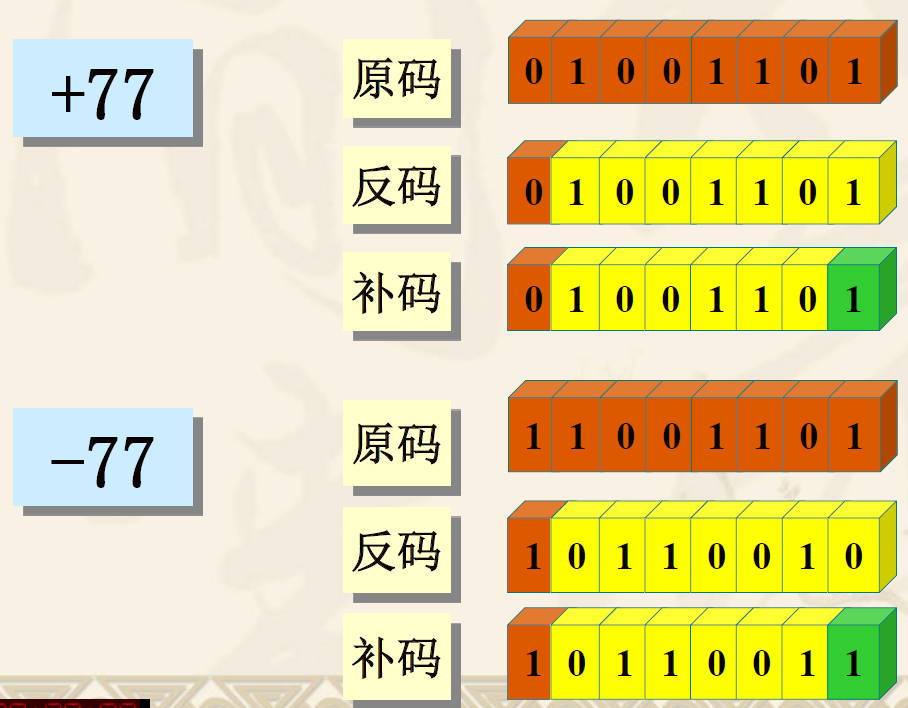
\includegraphics[scale=0.25]{2}
\end{frame}

\begin{frame}{ASCII编码表$B_6B_5B_4B_3B_2B_1B_0$}
\begin{columns}
	\column{0.7\textwidth}
	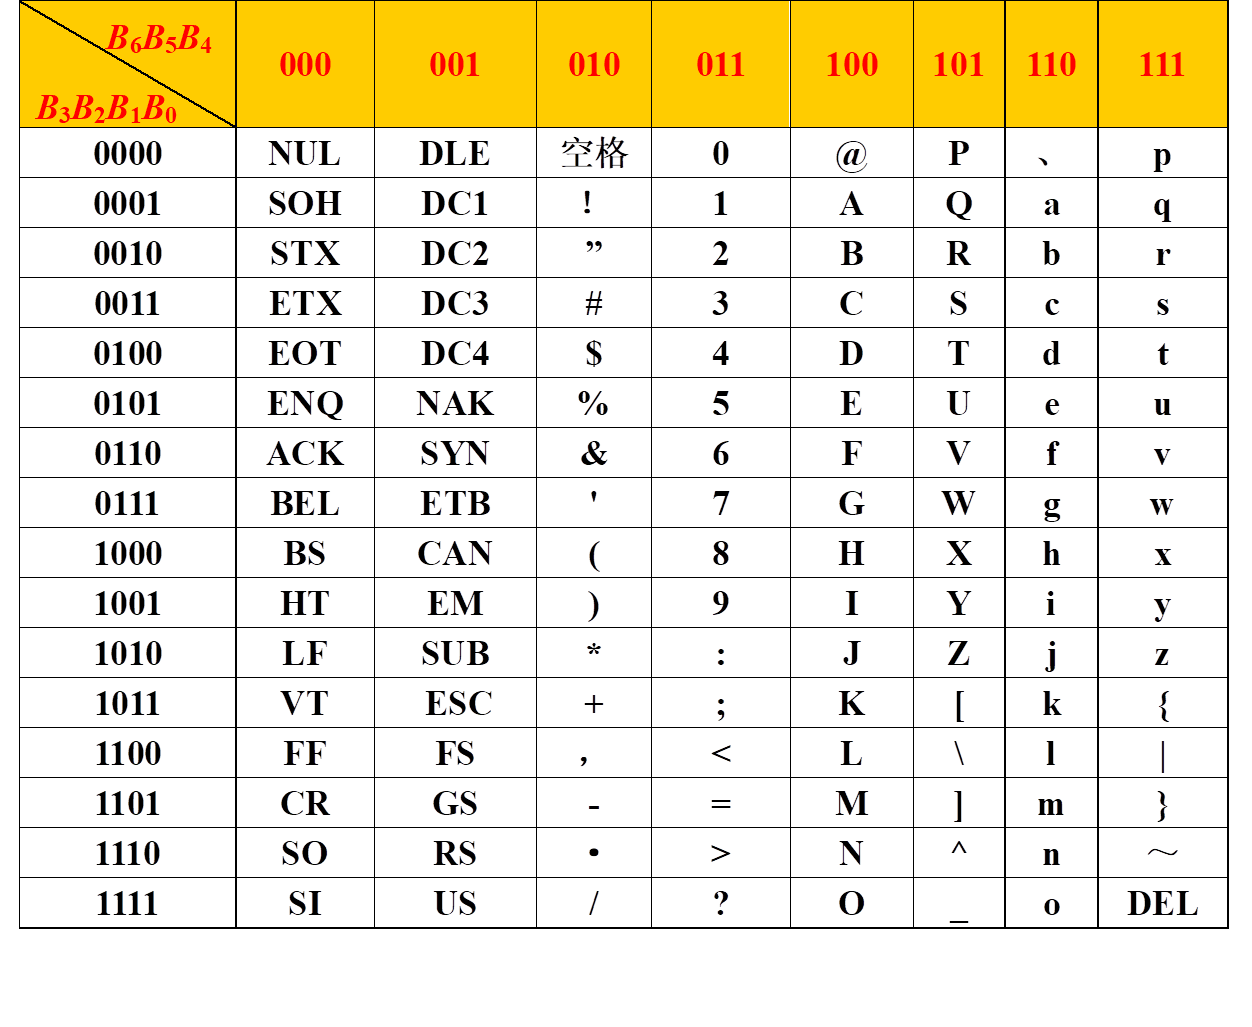
\includegraphics[scale=0.4]{ASCII}
	\column{0.3\textwidth}
	\begin{itemize}
		\item ASCII码连续排列 \\
		 `0'$\sim$`9', `A'$\sim$`Z', `a'$\sim$`z'
		\item 数字 = 编码值 - `0' \\
		 9=`9'-`0'
		\item 大小字符间隔: \\
		`a' - `A' = 32
	\end{itemize}
	
\end{columns}
\end{frame}

\section{C语言程序设计}

\begin{frame}{计算机程序}

\includegraphics[scale=0.4]{program1}
\end{frame}

\begin{frame}{计算机语言}
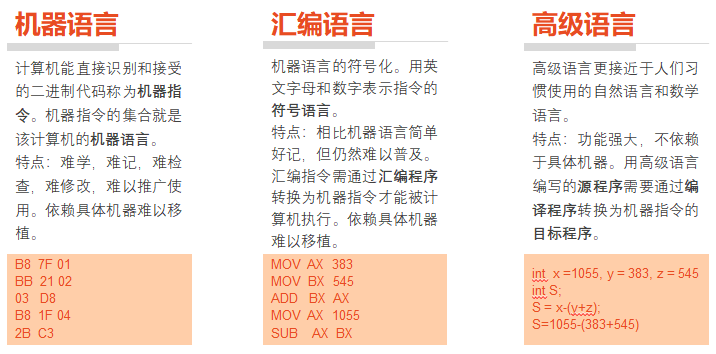
\includegraphics[scale=0.4]{program2}
\end{frame}

\begin{frame}{高级语言的发展}
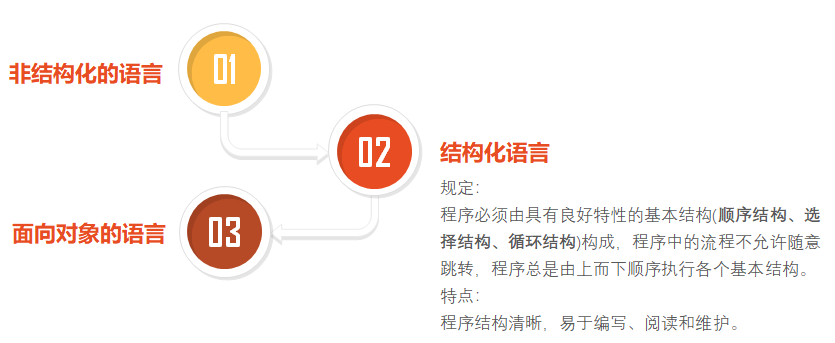
\includegraphics[scale=0.4]{program3}
\end{frame}

\begin{frame}{C语言的特点}
\begin{enumerate}
	\item 语言简洁、紧凑,使用方便、灵活
    \item 运算符丰富
    \item 数据类型丰富
    \item \textcolor{blue}{C语言是完全模块化和结构化的语言}\\
          具有结构化的控制语句(顺序、选择、循环结构)\\
          用函数作为程序的模块单位,便于实现程序的模块化
    \item \textcolor{blue}{兼具高级语言和低级语言的功能}\\
          允许直接访问物理地址\\
          能进行位(bit)操作\\  
          能实现汇编语言的大部分功能\\
          可以直接对硬件进行操作        
\end{enumerate}
\end{frame}

\begin{frame}{程序设计的任务}
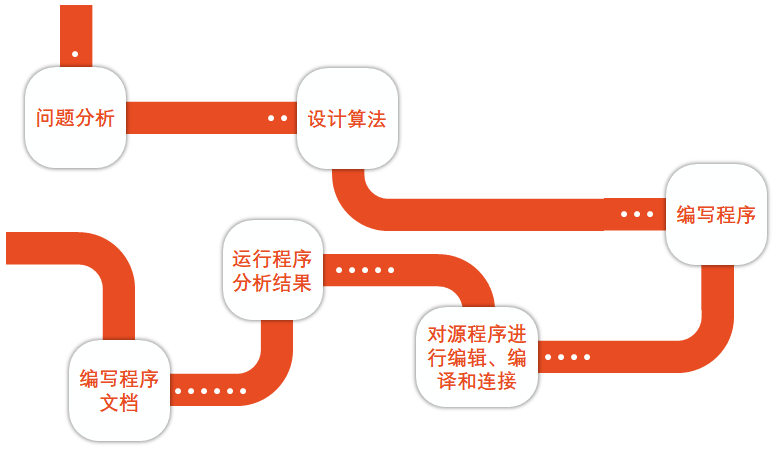
\includegraphics[scale=0.4]{program}
\end{frame}

\begin{frame}[fragile]{第一个C语言程序}
    \begin{lstlisting}
    #include<stdio.h>            // standard input/output编译预处理指令
    int main()                   // 主函数
    {                            // 函数开始标志
       printf("Hello World!");   // 输出一行信息
       return 0;                 // 函数执行完毕返回函数值0
    }                            // 函数结束标志
    \end{lstlisting}
\end{frame}

\begin{frame}[fragile]{求两个整数之和}
\begin{lstlisting}
#include<stdio.h>            // standard input/output编译预处理指令
int main()                   // 主函数
{                            // 函数开始标志
   int a,b,sum;           // 定义a,b,sum为整型变量
   a=123;                 // 对a,b赋值
   b=456;
   sum=a+b;              // 计算a+b, 并把结果存放在变量sum中
   printf("sum is %d\n",sum);   // 输出结果
   return 0;                 // 函数执行完毕返回函数值0
}                            // 函数结束标志
\end{lstlisting}
\end{frame}

\begin{frame}{运行C程序的步骤与方法}
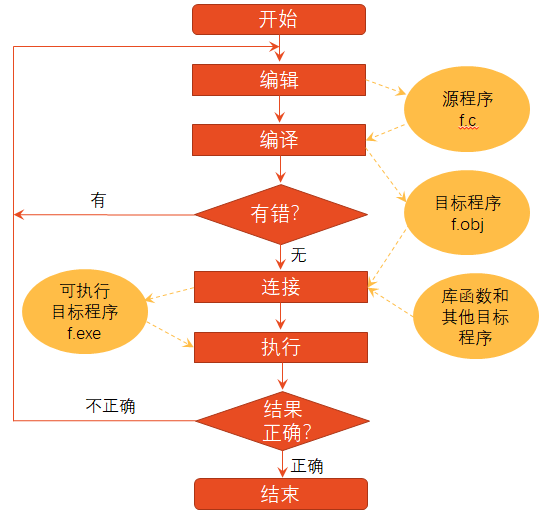
\includegraphics[scale=0.45]{program4}
\end{frame}

\begin{frame}{集成开发环境---编译系统}
\begin{itemize}
	\item Bloodshed Dev-C++ 
	\item Turbo C
	\item Visual C++6.0 
	\item Visual Studio(VS2015,VS Community 2019等)
\end{itemize}
\end{frame}

\begin{frame}{Bloodshed Dev-C++集成开发环境}
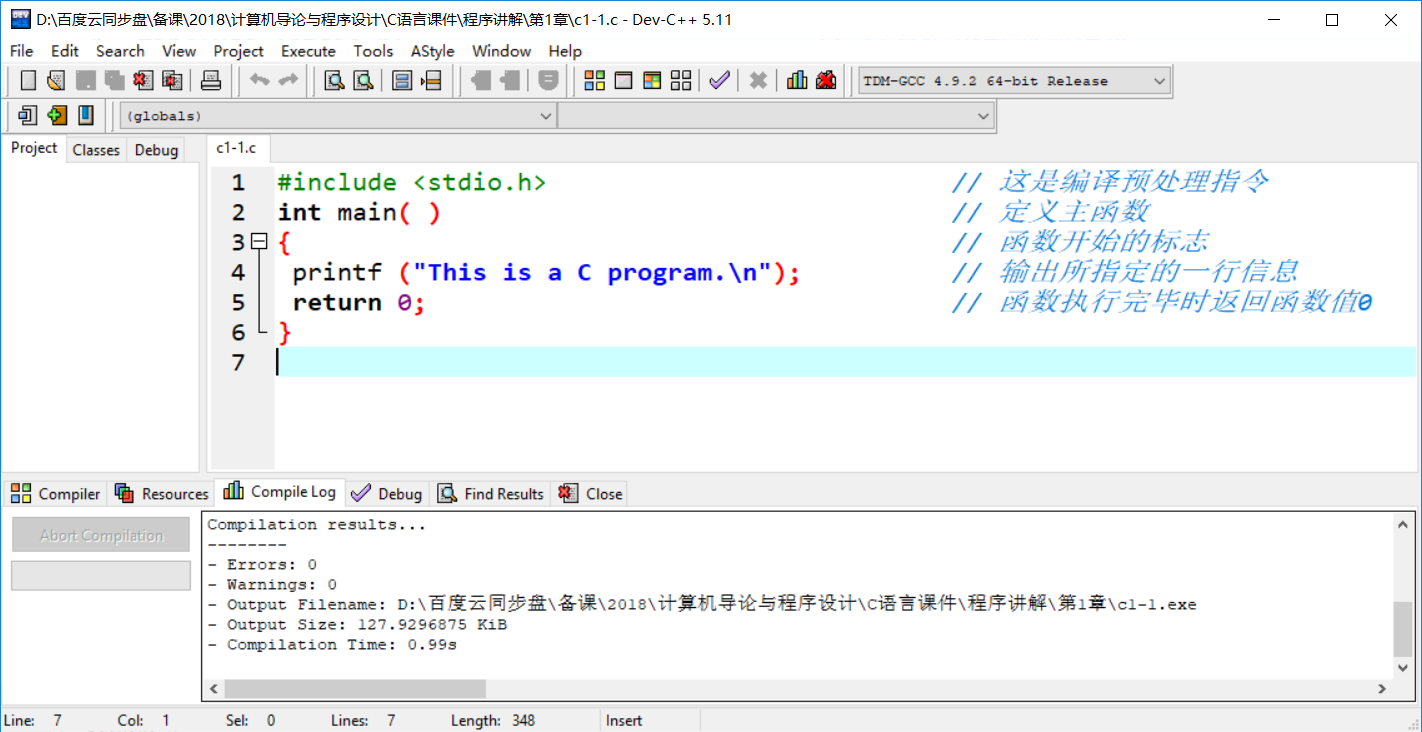
\includegraphics[scale=0.3]{DevCpp}   
\end{frame}

\begin{frame}{Bloodshed Dev-C++集成开发环境}
\begin{itemize}
	\item 选择“文件”菜单,选择“源文件”, 编辑程序。
	\item 保存时,保存为 .cpp或 .c文件。
	\item 选择“编译和运行”菜单,生成.exe文件,运行程序。  
\end{itemize} 
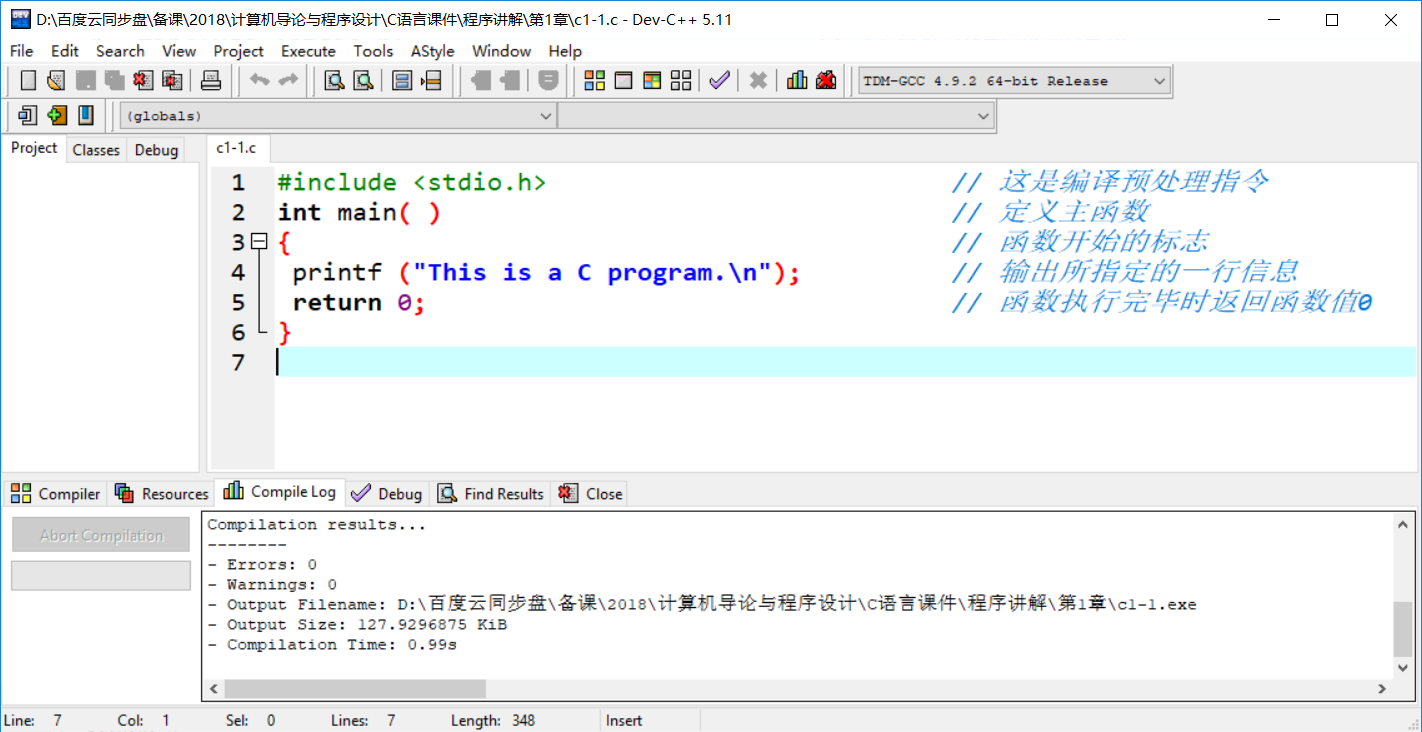
\includegraphics[scale=0.2]{DevCpp}   
\end{frame}